\date{\today}

%\documentclass[journal=jacsat,manuscript=communication,layout=twocolumn]{achemso}
%\documentclass[jctcce,letterpaper,twocolumn,floatfix,preprintnumbers,superscriptaddress]{revtex4}
% \documentclass[12pt,preprint,aps,prb]{revtex4}
% \documentclass[aps,preprint,showpacs,superscriptaddress,groupedaddress]{revtex4}  % for double-spaced preprint
\documentclass[aps,pra,twocolumn,superscriptaddress,groupedaddress]{revtex4}  % for review and submission
\usepackage{dcolumn,graphicx,amsmath,amssymb,algorithm,algpseudocode}
\usepackage{mathtools}
\usepackage{xcolor}
\usepackage{todonotes}
\usepackage{qcircuit}
\usepackage{subcaption}

\newcommand{\total}{\mathrm{d}}
\newcommand{\ud}{\mathrm{d}}
\newcommand{\erf}{\mathrm{erf}}
\newcommand{\erfc}{\mathrm{erfc}}
\newcommand{\diff}[2]{\frac{\ud {#1}}{\ud {#2}}}
\newcommand{\pdiff}[2]{\frac{\partial #1}{\partial #2}}

\begin{document}

\definecolor{brickred}{rgb}{.72,0,0} 
\definecolor{darkblue}{rgb}{0,0,0.5} 
\definecolor{darkgreen}{rgb}{0,0.5,0} 

\title{
Optimizing the Production of Test Vehicles: Classical Solutions Today and Hybrid Quantum/Classical Solutions Tomorrow
}

\author{Robert M. Parrish}
\email{rob.parrish@qcware.com}
\author{Rachael Al-Saadon}
\affiliation{
QC Ware Corporation, Palo Alto, CA 94301, USA 
}


\begin{abstract} 
A complete and completely classical solution of the industrial challenge problem
is presented.  Additional quantum/classical algorithmic gains are potentially
possible for harder future versions
of this problem experiencing geometric frustration - we propose a specific
research direction along these lines using a QC Ware specialty of quantum number
preserving gate fabric circuits to solve a key part of such a hybrid solution.
\end{abstract}

\maketitle

\section{Phase 1 Results}

The problem statements variously ask for optimization of the constituents of a
set or ``constellation'' of $n_{\mathrm{C}}$ test vehicles, with each test
vehicle taken from a state space of $\sim 469$ binary dimensions called
``features'' (this and other dimensions quoted below to vary in future problem
sizes), and with each test vehicle satisfying hard ``feature-group'' and
``type-build rule'' constraints corresponding to $\sim 25$ basic test vehicle
types. The problem statements, predicated by the hard constraints,
specifically ask for (1) \textbf{SAT:} For a given $n_{\mathrm{C}}$, does there
exist, for a given set of $n_{\mathrm{test}} \sim 644$ tests depending through
binary expressions on the state space of each test vehicle, a set of
$n_{\mathrm{C}}$ test cars for which the $n_{\mathrm{test}}$ tests can be
separately evaluated, with the caveat that there need be a ``multiplicity'' of $K_I \sim 1-5$ distinct
test vehicles required to satisfy test $I$ for $I \in [0, n_{\mathrm{test}})$?
(2) \textbf{Weighted MAX-SAT:} For a given $n_{\mathrm{C}}$, what is the optimal
constellation of test vehicles such that the weighted sum of satisfied
$n_{\mathrm{test}}$ tests, each requiring $K_I$ distinct test vehicles, is
maximized? and (3) \textbf{Scheduling (not precisely specified):} For a given
set of $n_{\mathrm{test}}$ tests and corresponding set of $n_{\mathrm{C}}$ test
vehicles satisfying said tests including $\{ K_I \}$ multiplicity constraints in
a MAX-SAT formalism of (2), what is the optimal scheduling of said vehicles into
a test sequence with at most $n_{\mathrm{slot}} \sim 10$ tests performed on
distinct cars in each timeslot and with tests assigned to integer test groups
with definite sorting of test groups within each car?

A specific instance of the problem class described above was provided by BMW.
Taken naively, this problem instance involves binary optimization over a state
space of $\sim 469\times60 = 28140$ binary variables (plus additional state
space variables for scheduling), i.e., a state space of $2^{28140} \sim
10^{6574}$ dimensions, with hard constraints and fairly generic logical
expressions needed to specify constraints and objective function values.  As
stated by BMW (quotes from the problem statement in italics): ``\textit{The
provided description is based on the actual numbers and constraints formulated
for this model. It, thus, represents the real complexity arising in a productive
setting.}''

Within the problem statement document, solutions to the above problems were
attempted using existing industry-standard SAT solvers and constraint
satisfaction solvers. The SAT problem of (1) was easily solved:
``\textit{For 100 cars, the problem can be solved in a few seconds. A linear search counting down
from 100 revealed the solution that at least 60 cars are needed to perform all the specified
750 tests.}''
However the weighted MAX-SAT problem of (2) was not solvable:
``\textit{On the other hand, the MAX-SAT problem was not solvable in a reasonable time with the
chosen approach.}''
Additionally, the scheduling problem of (3) was not solvable:
``\textit{[O]n the test laptop, the full problem with 700 tests wasn't solvable in less than 24
hours.}''

\begin{figure*}[ht]
\begin{center}
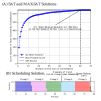
\includegraphics[width=4in]{figures/phase1/solution.pdf}
\caption{Characteristics of QC Ware solutions to the ``optimizing the production
of test vehicles'' BMW quantum computing challenge problem. (A) Solutions
to the MAX-SAT, and by corollary, SAT variants of problem variants (2) and (1),
respectively. (B) Solution to the scheduling problem variant (3).}
\label{fig:solution}
\end{center}
\end{figure*}

\textbf{We provide what we believe under the rules of the problem statement
represents a complete and tangible classical solution to all three specified
problem variants.} 
The characteristics of our solution are presented in Figure \ref{fig:solution}
and the specific solution data and corresponding code are present in our
publicly-available repository at
\href{https://github.com/qcware/bmw}{https://github.com/qcware/bmw}.
Specifically, we developed a custom C++/Python code library to represent the
details of the problem in a natural format. 
The combination of customized classical solution environment and high
performance implementation allows for very rapid exploration of the
hard-constraint-satisfying parameter space unique to this problem class.  Within
this environment, we developed a powerful and simple set of heuristics to
approximately solve the MAX-SAT variant of the problem. This heuristic MAX-SAT
solver produces nested constellations of test cars with increasing
$n_{\mathrm{C}}$ and concomitant increasing MAX-SAT scores. The MAX-SAT
solutions coming from this heuristic achieve saturation of all specified $644$
tests (including multiplicity considerations) at the same $n_{\mathrm{C}} = 60$
bound determined by standard SAT solvers for problem (1) in the problem
statement document. Thus our MAX-SAT solution provides a tight bound solution
for problem (1) in the process of providing approximate solutions for (2). For
values of $n_{\mathrm{C}} \ll 60$, we believe our heuristic MAX-SAT solutions
are within a few percent of the global optimum. For the scheduling problem of
(3) we develop additional heuristics to schedule the test sequence from the
MAX-SAT optimized constellation of $n_{\mathrm{C}} = 60$ cars while respecting
the hard constraints of distinct cars within each time slot, strict ordering of
randomly-specified test groups within cars, and separate cars used within the
multiplicity considerations of each test. With the multiplicity considerations
included, there are 766 separate test-car pairs required, mandating a
theoretical floor of 77 test slots. Our heuristic solution provides a nearly
dense scheduling with 78 test slots required, i.e., within 1.3$\%$ of dense
scheduling. In aggregate, the classical steps required to reach the
MAX-SAT/SAT/Scheduling solutions sum to roughly $5-10$ min total of wall time on
a 72-core AWS EC2 \texttt{c5n.metal} instance, representing $\sim \$0.30$ worth
of classical computing resources at present prices.

\section{Methods}

\subsection{C++/Python Environment}

To facilitate rapid exploration of the state space for this problem class, we
developed a custom C++11/Python3 library API linked by PyBind11. No additional
dependencies beyond standard C++11, Python3, and the header-only PyBind11 linker
layer are needed - i.e., we do not rely on third-party SAT solvers. This library
contains simple classes enumerating the natural representation of the problem
contents. For instance, a \texttt{SimpleBinaryExpression} class is implemented
to represent the concept of simple all/any binary expressions containing
arbitrary not predicates as encountered throughout the type build rules and the
test rules. Instances of this class store the state of, e.g., a given build rule
predicate or implication expression, and can efficiently check whether this
expression is satisfied for a given proposed vehicle configuration. Two
\texttt{SimpleBinaryExpression} objects are further stacked in a
\texttt{SimpleBinaryImplication} object to represent the predicate and
implication of each type build rule. Multiple \texttt{SimpleBinaryExpression}
objects are chained together in a \texttt{FirstOrderAllBinaryExpression} object
to represent the parenthesized binary expressions present in each test rule.
Additional data structures are constructed to uniquely represent the type
feature groups, the type-specific build rules, the full set of test rules and
corresponding multiplicities, eventually yielding a complete C++ representation
of the full problem. The critical configuration state space of each test vehicle
is efficiently represented by the \texttt{std::vector<bool>} concept, i.e., each
proposed test vehicle is represented by a \texttt{std::vector<bool>} containing the
states of the $\sim 469$ features of each vehicle.
 The entire library is reflexively exposed to Python3 through PyBind11 to merge
the effortless development of Python (i.e., regex for data parsing, short python
scripts to manage various experiments, compile-free debugging through python
printing) with the speed of compiled C++ for rate-limiting operations. The use
of C++ also facilitates the use of single-node parallelism through OpenMP
threading.

\subsection{Test Vehicle Seeds}

One might expect that the guess of $\vec 0$ (i.e., all features turned off)
would yield an acceptable starting guess for a test vehicle configuration.
However, already at $\vec 0$ some of the type build rules are violated, meaning
that $\vec 0$ is outside of the hard constraint space. Moreover, we have
empirically found that some of the $\sim 644$ test rules are rather hard to find
without specific direction within the constraint space. Therefore, to seed a
starting pool of test vehicles, we adopt the following procedure:
\begin{enumerate}
\item For each test rule, we generate a seed test vehicle that satisfies this
test rule with a randomly selected type.
\item To generate this vehicle, we first flip the required features on to
satisfy the test rule. 
\item The active test rule features are then ``masked'' meaning that they are
frozen in current values satisfying the test rule throughout all future steps.
\item In the non-masked features, we then chase constraints until we arrive at a
valid car satisfying the type build rules.
\item If this procedure fails for a given randomly selected type, we randomly
select another type and repeat ad infinitum.
\end{enumerate}
At the end of this procedure we have a pool of $\sim 644$ test vehicles which
are largely ``featureless'' meaning that only the minimal number of features
have been activated to satisfy the test and chase the constraints into the valid
type build rule space. All test rules are present in at least one test vehicle in this
starting pool.

\subsection{MAX-SAT Optimization}

We start from the empty constellation $n_{\mathrm{C}} = 0$. To update this
constellation to $n_{\mathrm{C}} = 1$, we adopt the following procedure:
\begin{enumerate}
\item For each of the $\sim 644$ test vehicles in the candidate pool, we
perform several tens of thousands of directed Monte Carlo moves designed to
improve the number of rules simultaneously satisfied by the test vehicle, while
respecting the hard constraints. The Monte Carlo moves are described below.
\item We add to the constellation the single car from the updated candidate pool
that maximally increases the number of satisfied tests in the constellation.
\item We update the test set used to direct the Monte Carlo moves in Step 1 to
include only those rules which are unsatisfied by the current constellation.
\item We iterate this procedure until all test rules are satisfied, increasing
the constellation size $n_{\mathrm{C}}$ by one test vehicle per iteration.
\end{enumerate}
At the end of this procedure, we have a set of $n_{\mathrm{C}}$ nested
constellations each of which is a local approximant to the MAX-SAT [Problem (2)]
solution of corresponding constellation size. Once we obtain a constellation
that saturates all tests, we have an upper bound for the SAT solution [Problem
(1)] which turns out to be tight for the specifics of this problem instance.

\subsection{Masked Distance-2 Monte Carlo Moves}

One of the particular specialties of our approach lies in the strength of our
Monte Carlo moves. We adopt the following procedure:
\begin{enumerate}
\item For each test vehicle in the candidate pool, we randomly select two
feature groups to vary.
\item For each of these feature groups we move with equal probability to
deactivate the feature group or to active a random feature index within the
group.
\item We check if the proposed move satisfies the type build rules and return to
1 if not.
\item We check if the proposed move would perturb the masked features discussed
in the previous section, and return to 1 if so. 
\item At this point, we know that the proposed test vehicle is valid and has not
moved a masked feature. If this proposed test vehicle improves the number of
satisfied tests in the active test set, we accept the updated vehicle and return
to 1. Else we reject the proposed test vehicle and return to 1.
\item We loop some user-specified number of iterations, usually on the order of
tens of thousands.
\end{enumerate}

There are several key observations that guided this heuristic choice of Monte
Carlo move scheme:
\begin{itemize}
\item These moves always remain on the constraint space.
\item These moves move by feature group rather than binary variables, and
therefore automatically satisfy the feature group constraint. Direct moves in
binary variables would have vanishing probability of satisfying the feature
group constraints.
\item Distance-2 moves are much more likely to be interesting and valid than
distance-1 moves. E.g., the activation of a single feature group often implies
the activation of another feature group through the type build rules. Such
implications can be satisfied with reasonable probability with distance-2 moves,
but are often unreachable with a sequence of distance-1 moves.
\item The acceptance of moves based on increased test set scores promotes a
compounding improvement of the test vehicle through the iterative procedure.
\end{itemize}

This procedure is implemented within C++, which treats the involved logic almost
natively. As such, we obtain orders of magnitude improvement over a
corresponding Python implementation of this portion of the approach.
Additionally, this stage of the procedure is embarrassingly parallel across the
$\sim 644$ test vehicles in the candidate pool. We parallelize this with OpenMP,
with dynamic scheduling invoked to attempt to load balance across the
anisotropic task sizes encountered.

Note that the efficiency of moves in this scheme relies on the concept that the
feature groups of the test vehicles are disjoint. This was not actually the case
in the original problem statement, due to a single collision between two feature
groups. We adjusted the problem statement to redefine two of the feature group
boundaries and to apply additional build constraint rules to yield an entirely
equivalent isomorphic representation of the problem. See the Appendix for
additional details.

\subsection{Scheduling}

For scheduling, we were initially considering doing some rather exotic work
involving global optimization, i.e., building a different constellation of test
vehicles that would be more optimized for the scheduling objective function than
for the MAX-SAT objective function. However, we started by exploring an extremely
simple greedy approach involving attempting to schedule our existing SAT/MAX-SAT
constellation of $n_{\mathrm{C}} = 60$ test vehicles, and found that it produced
almost dense packing. Therefore, we will only explain the latter approach here. 

The scheduling heuristic approach works as follows:
\begin{enumerate}
\item We first sort the test rules by test group (first priority) and by
number of required cars for the test (second priority).
\item We traverse the current priority-sorted test set.
\item For each test, we identify and randomly sort the list of cars which
satisfy the test.
\item For each car in this list, we attempt to add the car to the current time
slot, continuing deeper into the car list if the car already exists in the
current time slot, if the car has already been used previously for this test
(for multi-car tests), or if the car has already been used for a lower-priority
test group. As soon as we find a valid car, we break out of the loop over the
car list.
\item If no test-car pair can be added to the current slot, we ``nuke'' the slot
and kick it onto the schedule with no-ops (i.e., empty time/engineer slots) inside. 
\item If the addition of a car saturates the number of engineer slots, we kick
the slot onto the schedule.
\item We check if the addition of a car saturates a test rule, and update the
test rule set to remove this rule if so.
\item We iterate from 2 until all test rules are satisfied, as evidenced by the
active test set becoming empty.
\end{enumerate}

There is a small chance that this algorithm will enter an infinite loop where a
critical car is greedily used for a lower-priority test, and therefore cannot be
used for a higher-priority test. We have encountered this failure case in only
about 15$\%$ of runs. The existence of even a single successful run producing a
dense schedule obviates this concern. 

Note that we find the absence of specified test groups in the problem
specification to be a major weakness of this part of the challenge. We generated
test groups ranging from 1 to 5 from random integers as sketched in the problem
statement. We did this exactly once using \texttt{numpy.random.randint} and
stored the values in our github repository - i.e., we generated what we feel is
a fair test and then froze it. Note also that we elected to define the priority
order to be sorted from $1$ to $5$ rather than from $5$ to $1$ in the problem
statement for aesthetic reasons - as these values are isotropically randomly
generated this makes no difference in problem structure.

\section{Toward Hybrid Quantum/Classical Approaches}

\subsection{Motivation}

We view the above full solutions as an unexpected
\emph{fait accompli} obtained during our formulation of a submission for this
challenge. Despite the formidable presentation of
this problem [as evidenced by the inability of the BMW working group to provide
a solution for problem variants (2) and (3) with conventional techniques], this
problem is not so hard as it looks. In particular, there seems to be only a
moderate amount of ``geometric frustration'' between test vehicles. This concept
of geometric frustration has many potential manifestations, all stemming from
the basic idea that local moves to optimize one subset of the problem could
easily have severely penalized the quality of the global solution. For instance,
focusing on MAX-SAT, it could well have been the case that feature choices on
candidate test vehicles were so tightly correlated through test case
satisfaction that attempts to locally maximize the solution quality for each
proposed single test vehicle addition to the constellation would severely negatively
impact the MAX-SAT score for larger values of constellation size
$n_{\mathrm{C}}$. This might manifest as a problem instance where no single test
vehicle in the ideal global solution constellation is a ``hero'' individually
satisfying a relatively large number of tests (note that all of our current
solution test vehicles are heroes!). Instead each test vehicle in the ideal
solution constellation might satisfy only something on the order of
$n_{\mathrm{test}} / n_{\mathrm{C}}$ cars, with the particular test cluster
satisfied for by each test vehicle determined by a very brittle set of many-body
correlations with the active features sets across all test vehicles in the
constellation. Such a case would stymie essentially all heuristic optimization
approaches that we can evision.

A geometrically frustrated problem instance of this type is not hard to imagine
occurring in real engineering practice. In fact, we would argue that such
geometric frustration is already present in the current problem instance, albeit
to a low enough degree that some halfway clever heuristics and the big hammer of a
\texttt{c5n.metal} node can defeat such geometric frustration.  In particular,
as the feature groups, build rules, and test sets all grow in both size and
complexity in future practice at BMW, we will likely see cases that are highly
resilient to direct solution by local heuristics.

Below, we propose a specific directed research project to develop novel hybrid
quantum/classical algorithms to target such frustrated MAX-SAT problems. Key to
our approach is the idea that one should use the CPU (or other high-performance
classical computing resources) and QPU separately for what each are best at. As
such, we propose a two-stage approach where one first uses the CPU to generate a
large, diverse, and structured candidate pool of cars (dealing with the hard
build constraints on the cars on the CPU) and then selecting the best
constellation of $n_{C}$ test cars from this pool by using the QPU to solve a
variant of MAX-COVER. This variant of MAX-COVER is an interesting and
non-trivial extension of standard MAX-COVER that represents a total
Hamming-weight-constrained polynomial binary optimization problem (a specific
PCBO problem). 

Before discussing the proposed approach, we will briefly discuss a red herring
approach that will serve to contrast with our selected approach:

\subsection{A Path to Avoid}

It is highly tempting to map the binary state space of the MAX-SAT variant of
the problem to the qubits or qudits of a quantum device. This mapping would
provide the most direct encapsulation of the problem on the quantum hardware
and would retain the conceptually sacred possibility of an exact global optimum.
Conceptually, one would create a quantum superposition over all possible binary
strings in the state space, and then start applying MAX-SAT-Hamiltonian-aware
methods like quantum amplitude amplification (using either traditional deep
quantum phase estimation circuits or a variant of the new short-depth maximum
likelihood estimation, Grover zeroing, or Chinese remainder theorem circuit
schedules), QAOA, or VQE to boost the observation probability of the global
optimum or other local optima. One could immediately improve this idea by either
conceptually or physically using qudits to represent each feature group - this
would drastically reduce the search space size and simultaneously mitigate
issues with the feature group constraints.

We do not recommend pursuing any approach along these lines for exactly one reason:
test vehicle build constraints. These constraints severely limit the valid state
space of the test vehicles and are posed as generic predicate/implication binary
logic statements involving up to dozens of simultaneous variables per expression. Such
constraints are completely alien in a quantum computing context, in the same way
that mapping a deeply serial code to a GPU is a technical non-starter.
Therefore, we see no viable path (even for error-corrected quantum  approaches in
the $\geq$decade timeframe) to develop general purpose quantum circuits that can
provide powerful moves within the Hilbert space while simultaneously respecting
these generic build rules.

\subsection{A Path to Take}

We instead propose a hybrid quantum/classical approach to the geometrically frustrated MAX-SAT
problem. The approach works as follows:
\begin{enumerate}
\item Use classical high performance computing resources such as extensions of
our existing methodology to build a large, diverse, and highly structured pool
of $\sim 10^{2}$ to $\sim 10^{6}$ candidate test vehicles. This pool generation approach
can be tuned for various frustration cases, e.g., providing penalties for
``hero'' test vehicles, providing repulsive terms between test vehicles with overlapping
feature sets, or encouraging small groups of test vehicles to work together to
realize tests with high multiplicities.
\item Use novel symmetry-preserving constrained binary optimization optimization
approaches on quantum hardware to solve the modified MAX-COVER problem of
selecting the optimal constellation of $n_{C}$ test vehicles from the candidate
pool. 
\item Perform additional heuristic refinement on classical resources to further
increase the MAX-SAT score.
\end{enumerate}

\subsection{The Quantum Problem}

The modified MAX-COVER problem that represents the basic task of the quantum
hardware in our hybrid method has the following two compelling features: (1) the
problem maps much more naturally to a qubit device than the approach discarded
in the previous section and (2) the problem has an extremely interesting global
Hamming weight constraint structure that merits additional quantum algorithm
development, i.e., there is something new, tangible, and valuable to be done
here on the quantum algorithms research side. 

Specifically, we have a binary state space of $n_{P}$ binary variables, where
$n_{P} \sim 10^{2} - 10^{6}$ is the number of test vehicles in the candidate
pool. We are asked to produce a $n_{P}$-dimensional binary string with Hamming
weight (total number of 1-state bits) $n_{C}$, where the $n_{C}$ 1-state bits
identify the pivots of the test pool to place into the test constellation. This
binary string is to be optimized to maximize the number of satisfied test cases
in the constellation, including mutliplicity considerations. This last
consideration generalizes the problem beyond standard MAX-COVER somewhat,
implying some extensions to the Hamiltonian considerations that we will consider
in future work. 

The most interesting feature of the problem is the total Hamming weight
constraint. This formally reduces the dimension of the search space from
$2^{n_{P}}$ to ${n_{P} \choose n_{C} }$, which is still a roughly exponentially
large search space. Standard heuristics for MAX-COVER will likely fail in this
environment due to the same geometric frustration between choices that motivated
our basic consideration of a hybrid quantum/classical algorithm. The challenge
at this point is to craft a quantum optimization algorithm that respects the
hard Hamming weight constraint while also providing strong optimization power.
Some existing approaches have discussed this case, such as a variant of the
quantum alternating operator ansatz (QAOA) with ring or complete graph mixers
\cite{cook2020quantum},
or the mixer-phaser ansatz for QAOA with hard Hamming constraints \cite{larose2021mixer}. Both of these
methods share the common traits that they start from Dicke states (essentially
the usual $|+\rangle$ state of equal amplitudes on all state space
configurations, but restricted to preserve target Hamming weight), and then use
arrays of 2-qubit XY mixer gates (similar to the ``reversible beamsplitter or RBS
gates'' of quantum optics'' or the ``Givens gates'' of quantum chemistry) to
provide Hamming-wight-preserving exploration through the Hilbert space during
the QAOA optimization process. It might be possible to directly implement one of
this existing methods to solve the MAX-COVER problem for our problem instance.
However, we note that there exist several potential problems with these
proposed ansatze. Most tangibly (1) it is well known that networks of Givens or
similar gates do not provide full entangling power across the
Hamming-weight-preserving Hilbert space, and therefore may not be able to
provide quantum advantage when used as QAOA elements and (2) some of the most
promising variants of the existing approaches, such as the complete graph XY
mixers use highly nonlocal pairs of non-adjacent qubits that may be
prohibitively difficult to implement on near-term quantum devices with limited
qubit connectivity. We propose an avenue of research that goes somewhat beyond
these existing methods, and that works to directly confront these two major
issues: the adoption of universal Hamming-weight-preserving gate fabrics into an
extended version of QAOA or VQE that can provide full universality within the
Hamming-weight-preserving subspace while simultaneously being amenable to
implementation on NISQ-era quantum devices as a simple 3-local nearest-neighbor
gate fabric.  

These Hamming-weight-preserving quantum number gate fabrics were noticed as an
aside during a collaborative effort between QC Ware Corp. and Covestro
Deutschland AG to develop universal but simple gate fabric circuits for the
simulation of fermions in the context of quantum chemistry \cite{anselmetti2021local}. Fermions exhibit
numerous symmetry constraints which must be respected during quantum algorithms simulating
these fermions, and one of these symmetries in Hamming weight. Therefore, as an
intermediate to full the full fermionic gates that were the major finding of
Ref. \citenum{anselmetti2021local}, we considered the prerequisite question of the minimal circuit that is
universal for total Hamming weight while also preserving a semblance of
simplicity and linear locality. As is well-known in the literature, we noted
that the two-qubit fabric of Givens gates as in Figure \ref{fig:H1} (similar to
the XY mixers discussed above) are not universal, but an extension of this
concept to a local fabric of three-qubit Hamming-weight-preserving gates as
depicted in Figure \ref{fig:H2} achieves universality while preserving the
global Hamming weight constraint. 

\begin{figure}[b]
\centering
\begin{equation*}
\begin{array}{l}
\Qcircuit @R=0.3em @C=0.3em @!R {
% \lstick{|0\rangle}
 & \multigate{1}{\mathit{H}(4)}
 & \qw
 & \multigate{1}{\mathit{H}(4)}
 & \qw
 & \qw \\
% \lstick{|1\rangle}
 & \ghost{\mathit{H}(4)}
 & \multigate{1}{\mathit{H}(4)}
 & \ghost{\mathit{H}(4)}
 & \multigate{1}{\mathit{H}(4)}
 & \qw \\
% \lstick{|2\rangle}
 & \multigate{1}{\mathit{H}(4)}
 & \ghost{\mathit{H}(4)}
 & \multigate{1}{\mathit{H}(4)}
 & \ghost{\mathit{H}(4)}
 & \qw \\
% \lstick{|3\rangle}
 & \ghost{\mathit{H}(4)}
 & \multigate{1}{\mathit{H}(4)}
 & \ghost{\mathit{H}(4)}
 & \multigate{1}{\mathit{H}(4)}
 & \qw \\
% \lstick{|4\rangle}
 & \multigate{1}{\mathit{H}(4)}
 & \ghost{\mathit{H}(4)}
 & \multigate{1}{\mathit{H}(4)}
 & \ghost{\mathit{H}(4)}
 & \qw \\
% \lstick{|5\rangle}
 & \ghost{\mathit{H}(4)}
 & \qw
 & \ghost{\mathit{H}(4)}
 & \qw
 & \qw \\
}
\end{array}
\ldots
\phantom{}
\not\cong
\phantom{}
\begin{array}{l}
\Qcircuit @R=0.3em @C=0.3em @!R {
% \lstick{|0\rangle}
 & \multigate{5}{\mathit{H}(2^6)}
 & \qw \\
% \lstick{|0\rangle}
 & \ghost{\mathit{H}(2^6)}
 & \qw \\
% \lstick{|0\rangle}
 & \ghost{\mathit{H}(2^6)}
 & \qw \\
% \lstick{|0\rangle}
 & \ghost{\mathit{H}(2^6)}
 & \qw \\
% \lstick{|0\rangle}
 & \ghost{\mathit{H}(2^6)}
 & \qw \\
% \lstick{|0\rangle}
 & \ghost{\mathit{H}(2^6)}
 & \qw \\
}
\end{array}
\end{equation*}
\begin{equation*}
\begin{array}{l}
\Qcircuit @R=0.3em @C=0.3em @!R {
 & \multigate{1}{H(4)}
 & \qw \\
 & \ghost{H(4)}
 & \qw \\
}
\end{array}
\coloneqq
\begin{array}{l}
\Qcircuit @R=0.3em @C=0.3em @!R {
 & \gate{R_{y} (+\pi / 4)}
 & \ctrl{1}
 & \gate{R_{y} (+\lambda / 2)}
 & \ctrl{1}
 & \gate{R_{y} (-\pi / 4)}
 & \qw \\
 & \gate{R_{y} (+\pi / 4)}
 & \ctrl{-1}
 & \gate{R_{y} (-\lambda/2)}
 & \ctrl{-1}
 & \gate{R_{y} (-\pi / 4)}
 & \qw \\
}
\end{array}
\end{equation*}
\begin{equation*}
=
\left [
\begin{array}{rrrr}
1 & & & \\
 & c & +s & \\
 & -s & c & \\
 & & & 1 \\
\end{array}
\right ]
:
\
\begin{array}{l}
c \coloneqq \cos(\lambda/2)
\\
s \coloneqq \sin(\lambda/2)
\\
\end{array}
\end{equation*}

\caption{From Ref. \citenum{anselmetti2021local}: Gate fabric attempt \emph{not}
universal for the Hamming-weight-preserving subgroup $\mathcal{H}(2^N)$
(sketched for $N=6)$.  The gate fabric is a 2-local-nearest-neighbor
tessellation of alternating even and odd qubit-pair 1-parameter, 2-qubit
Hamming-weight-preserving $\hat H(4)$ gates.  The gate fabric exactly commutes
with the Hamming weight operator $\hat P \equiv \sum_{p} (\hat I - \hat Z_p) /
2$, but the gate fabric does not span $\mathcal{H}(2^N)$ for any depth.
}
\label{fig:H1}
\end{figure}

\begin{figure}
\centering
\begin{equation*}
\label{eq:SO2N-Hamming}
\begin{array}{l}
\Qcircuit @R=0.3em @C=0.3em @!R {
% \lstick{|0\rangle}
 & \multigate{2}{\mathit{H}(8)}
 & \qw 
 & \qw 
 & \qw 
 & \qw \\
% \lstick{|1\rangle}
 & \ghost{\mathit{H}(8)}
 & \multigate{2}{\mathit{H}(8)}
 & \qw 
 & \qw \\
% \lstick{|2\rangle}
 & \ghost{\mathit{H}(8)}
 & \ghost{\mathit{H}(8)}
 & \multigate{2}{\mathit{H}(8)}
 & \qw \\
% \lstick{|0\rangle}
 & \multigate{2}{\mathit{H}(8)}
 & \ghost{\mathit{H}(8)}
 & \ghost{\mathit{H}(8)}
 & \qw \\
% \lstick{|1\rangle}
 & \ghost{\mathit{H}(8)}
 & \multigate{2}{\mathit{H}(8)}
 & \ghost{\mathit{H}(8)}
 & \qw \\
% \lstick{|2\rangle}
 & \ghost{\mathit{H}(8)}
 & \ghost{\mathit{H}(8)}
 & \multigate{2}{\mathit{H}(8)}
 & \qw \\
% \lstick{|0\rangle}
 & \multigate{2}{\mathit{H}(8)}
 & \ghost{\mathit{H}(8)}
 & \ghost{\mathit{H}(8)}
 & \qw \\
% \lstick{|1\rangle}
 & \ghost{\mathit{H}(8)}
 & \qw 
 & \ghost{\mathit{H}(8)}
 & \qw \\
% \lstick{|2\rangle}
 & \ghost{\mathit{H}(8)}
 & \qw 
 & \qw 
 & \qw \\
}
\end{array}
\phantom{}
\ldots
\cong
\phantom{}
\begin{array}{l}
\Qcircuit @R=0.3em @C=0.3em @!R {
% \lstick{|0\rangle}
 & \multigate{8}{\mathit{H}(2^9)}
 & \qw \\
 & \ghost{\mathit{H}(2^9)}
 & \qw \\
 & \ghost{\mathit{H}(2^9)}
 & \qw \\
 & \ghost{\mathit{H}(2^9)}
 & \qw \\
 & \ghost{\mathit{H}(2^9)}
 & \qw \\
 & \ghost{\mathit{H}(2^9)}
 & \qw \\
 & \ghost{\mathit{H}(2^9)}
 & \qw \\
 & \ghost{\mathit{H}(2^9)}
 & \qw \\
 & \ghost{\mathit{H}(2^9)}
 & \qw \\
}
\end{array}
\end{equation*}
\begin{equation*}
\mathit{H} (8)
\coloneqq
\left [
\begin{array}{rrrrrrrrr}
1 & & & & & & & & \\
 & \color{brickred}{u_{00}^{1}} & \color{brickred}{u_{01}^{1}} & &
\color{brickred}{u_{02}^{1}} & & & & \\
 & \color{brickred}{u_{10}^{1}} & \color{brickred}{u_{11}^{1}} & &
\color{brickred}{u_{12}^{1}} & & & & \\
 & & & \color{darkblue}{u_{00}^{2}} & & \color{darkblue}{u_{01}^{2}} &
\color{darkblue}{u_{02}^{2}} & \\
 & \color{brickred}{u_{20}^{1}} & \color{brickred}{u_{21}^{1}} & &
\color{brickred}{u_{22}^{1}} & & & & \\
 & & & \color{darkblue}{u_{10}^{2}} & & \color{darkblue}{u_{11}^{2}} &
\color{darkblue}{u_{12}^{2}} & \\
 & & & \color{darkblue}{u_{20}^{2}} & & \color{darkblue}{u_{21}^{2}} &
\color{darkblue}{u_{22}^{2}} & \\
& & & & & & & & 1 \\
\end{array}
\right ]
\end{equation*}
\begin{equation*}
\hat u^{d}
\coloneqq
\exp(\hat x^{d})
\in 
\mathcal{SO}(3)
:
\
\hat x^{d\dagger}
=
-
\hat x^{d}
:
\hat x^{d}
\in
\mathbb{R}^3
\times
\mathbb{R}^3
, 
\
d \in [1, 2]
\end{equation*}
\caption{From Ref. \citenum{anselmetti2021local}: Gate fabric  universal for the Hamming-weight-preserving subgroup
$\mathcal{H}(2^N)$ (sketched for $N=9)$.  The gate fabric is a
3-local-nearest-neighbor tessellation of cascading qubit-triple 6-parameter,
3-qubit Hamming-weight-preserving $\hat H(8)$ gates. Each $\hat H(8)$ gate is
composed of a 3-parameter $\mathcal{SO}(3)$ rotation in the $d$-Hamming-weight
subspace, where $d \in [1, 2]$ for a total of 6 parameters. The gate fabric exactly
commutes with the Hamming weight operator $\hat P \equiv \sum_{p} (\hat I - \hat
Z_p) / 2$ and spans $\mathcal{H}(2^N)$ at sufficient depth.
}
\label{fig:H2}
\end{figure}

A tangible and potentially highly valuable research direction is to build an
extension of QAOA or VQE built around these three-qubit quantum number
preserving gates to address the MAX-COVER problem needed for our hybrid
quantum/classical solution to the geometrically frustrated test vehicle
production MAX-SAT problem. This is the basis of our research proposal to BMW.

\section{Phase 2 Results}

\begin{figure*}[ht]
\begin{center}
\includegraphics[width=4in]{figures/phase2/6-reduce-rules.pdf}
\caption{Result of reducing features of constellation generated in Phase 1.
         Blue indicates the number of test rules satisfied with the initial constellation
         generated in Phase 1 whereas red represents the results of Phase 2 reduction of
         feature set from the initial constellation from Phase 1.}
\label{fig:6-reduce}
\end{center}
\end{figure*}

\begin{figure*}[ht]
\begin{center}
\includegraphics[width=4in]{figures/phase2/2p-score.pdf}
\caption{Comparison of the results from Phase 1 and Phase 2 MAX-SAT. Phase 1 (blue) was
         carried out without feature restriction and Phase 2 (red) restricted the Hamming
         weight of each vehicle.}
\label{fig:solution2}
\end{center}
\end{figure*}

\begin{figure*}
  \centering
  \begin{subfigure}[b]{.475\textwidth}
    \centering
    % include first image
    \includegraphics[width=\textwidth]{figures/phase2/2-prod-hamming.pdf}  
    \caption{Phase 1 constellation Hamming weight.}
    \label{fig:sub-first}
  \end{subfigure}
  \hfill
  \begin{subfigure}[b]{.475\textwidth}
    \centering
    % include second image
    \includegraphics[width=\textwidth]{figures/phase2/2p-prod-hamming.pdf}  
    \caption{Phase 2 Hamming-weight constrained constellation Hamming weight.}
    \label{fig:sub-second}
  \end{subfigure}
  \vskip\baselineskip
  \begin{subfigure}[b]{.475\textwidth}
    \centering
    % include third image
    \includegraphics[width=\textwidth]{figures/phase2/2-prod-rules.pdf}  
    \caption{Phase 1 constellation test rules satisfied.}
    \label{fig:sub-third}
  \end{subfigure}
  \hfill
  \begin{subfigure}[b]{.475\textwidth}
    \centering
    % include fourth image
    \includegraphics[width=\textwidth]{figures/phase2/2p-prod-rules.pdf}  
    \caption{Phase 2 Hamming-weight constrained constellation test rules satisfied.}
    \label{fig:sub-fourth}
  \end{subfigure}
  \caption{Comparison of the results from Phase 1 and Phase 2. Plots (a) and (b) show the
           Hamming weight of each vehicle in the constellation. Plots (c) and (d) show the
           number of test rules satisfied per vehicle in the constellation.}
  \label{fig:fig}
\end{figure*}



\appendix
\newpage
\clearpage

\section{Phase 1: Details of Problem Refinement and Solution Validation}

\subsection{Feature Groups Collision Issue}

The efficient exploration of the state space in terms of moves in feature groups
requires that the feature groups be disjoint. We found that this was not the
case in the specified problem due to a collision between feature groups 40 and
41. To fix this issue, we modified these two groups and added additional type
build rules to produce an isomorphic variant of the problem with disjoint
feature groups. Details:

Group 40 (28 elements): \texttt{[245, 246, 247, 250, 251, 252, 253, 254, 255,
256, 266, 267, 268, 269, 270, 271, 272, 273, 274, 275, 276, 277, 278, 279, 280,
281, 282, 284]}

Group 41 (46 elements): \texttt{[245, 246, 247, 248, 249, 250, 251, 252, 253,
254, 255, 256, 257, 258, 259, 260, 261, 262, 263, 264, 267, 268, 269, 270, 271,
272, 273, 274, 275, 276, 277, 278, 279, 280, 281, 282, 283, 285, 286, 287, 288,
289, 290, 291, 292, 293]}

Union (48 elements): \texttt{[245, 246, 247, 248, 249, 250, 251, 252, 253, 254,
255, 256, 257, 258, 259, 260, 261, 262, 263, 264, 266, 267, 268, 269, 270, 271,
272, 273, 274, 275, 276, 277, 278, 279, 280, 281, 282, 283, 284, 285, 286, 287,
288, 289, 290, 291, 292, 293]}

Intersection (26 elements): \texttt{[245, 246, 247, 250, 251, 252, 253, 254,
255, 256, 267, 268, 269, 270, 271, 272, 273, 274, 275, 276, 277, 278, 279, 280,
281, 282]}

In Group 40 but not Group 41 (2 elements): \texttt{[266, 284]}

In Group 41 but not Group 40 (20 elements): \texttt{[248, 249, 257, 258, 259,
260, 261, 262, 263, 264, 283, 285, 286, 287, 288, 289, 290, 291, 292, 293]}

This is hugely vexing for efficient enumeration of group-feature-satisfying
vehicle candidates.

This can be overcome by (1) redefining Group 40 to be \texttt{[266, 284]} and
then (2) adding a new global (added for all types) rule to the type build rules:

\texttt{ F266 | F284 => !F245 \& !F246 \& !F247 \& !F250 \& !F251 \& !F252 \& !F253 \&
!F254 \& !F255 \& !F256 \& !F267 \& !F268 \& !F269 \& !F270 \& !F271 \& !F272 \& !F273 \&
!F274 \& !F275 \& !F276 \& !F277 \& !F278 \& !F279 \& !F280 \& !F281 \& !F282}

If the group features are chosen randomly, uniformly, and independently, this
rule has a probability of $2/(1+2)$ to be activated (if 266 xor 284 are true).
The probability of the rule being violated is $\sim 26/(1+46) \sim 0.55$.
Therefore the joint probability of the rule being activated and failing is
$(2/3) * (26/47) \sim 0.37$. Note that this high success probability is somewhat
accidental, and is only due to the fact that the in-40-but-not-in-41 subset is
small relative to the intersection \emph{and} the in-41-but-not-in-40 subset is
large relative to the the intersection. In future, it is recommended that
collisions between feature groups be avoided at all costs in the formulation of
this problem, insofar as is possible.

\subsection{Solution Verification}

A standalone Python code was used to verify that the solutions reported satisfy
both the buildability and test constraints.

The MAX-SAT heuristic produced a constellation of test vehicles with specified
active features. The test vehicles must comply with a set of buildability
constraints related (1) vehicle type, (2) feature group exclusivity, and
(3) configuration rules.

Each vehicle can be one of 25 types, which dictates allowed features. 
The type rules were sorted in a (\textit{number of types} $\times$
\textit{number of available features}) boolean array, with allowed features set
to True. For each vehicle in the solution constellation, if a feature was True,
it was compared to the allowed features for that vehicle type to assert that the
vehicle met type rules.

The feature groups constraints consist of 42 feature groups, which contain a set
of mutually exclusive features. For each test vehicle, one feature in the group can
be true. The feature groups were sorted in a (\textit{number of groups} $\times$
\textit{number of available features}) boolean array with each feature in the group
set to True. For each test vehicle, if a feature was True, the feature group for
which that feature was present was found and the bitwise AND was taken between
these two arrays, returning one True value if satisfied.

The set of test vehicles must also satisfy the configuration constraints. For a
given test vehicle type, a set of features is either forced and/ or forbidden
based on the presence and absence of specific features. There are 4032
configuration constraints in the problem. Each configuration rule was separated
into an initial condition and a forced implication. Theses were further reduced
to 'on' sets, 'off' sets, and sets where 'any' one feature can be true, all of
which were stored as True in boolean arrays. For each test vehicle, the
configuration rules associated with the vehicle type were evaluated. First the 
initial condition then forced implication was checked, in the same procedure
outlined below. (1) If the rule had a set of 'on' features, the logical AND of
the test vehicle features and 'on' features rule was computed. The number of
True values in the resultant array should equal those in the 'on' features array
if satisfied. (2) If the rule had a set of 'off' features, the array of features
for the test vehicle was inverted, so that 'off' features were set to True. Then
the logical AND was computed, which should have the same number of True elements
as the 'off' features array if satisfied. (3) If the rule had an 'any' set, where
one of the features must be true, the AND was taken between the 'any' features
array and the test vehicle features, which should return one True value.

For the scheduling solution, we verified that the results obey the scheduling
rules. The scheduling rules stipulate that there are up to 10 tests per day and
that each vehicle can undergo one test per day. We check that for each test day,
each vehicle index appears once. Next, each test is ranked in a group, and for
each test vehicle, it must undergo tests in order according to the test ranking.
To test that this condition is satisfied, we sort through the group rank of each
test vehicle. If a group index is out of order, we find which vehicle is in that
slot, and trace back all previous tests that the vehicle underwent. If the tests
for that specific vehicle are in order of ranking, the test set satisfies the test
group rank rules. Finally, each test requires a certain number of test vehicles.
For each test, we find and count all occurrences of that specific test and compare
it to the number required for that test. 

\section{Phase 2: . . .}

\end{document}
